\subsection*{Directed Graphs and Properties of Relations}
In Section~\ref{S:relations}, we used directed graphs, or digraphs, to represent relations on finite sets.  Three properties of relations were introduced 
in \typeu Activity~\ref*{PA:propsofrelaitons} and will be repeated in the following descriptions of how these properties can be visualized on a directed graph.  

Let $A$ be a nonempty set and let $R$ be a relation on $A$.
\begin{itemize}
\item  The relation  $R$  is 
\textbf{reflexive on}
\index{reflexive}%
\index{relation!reflexive on}%
 $\boldsymbol{A}$  provided that for each  
$x \in A$,  $x \mathrel{R} x$ or, equivalently,  $\left( {x, x} \right) \in R$.

This means that if a reflexive relation is represented on a digraph, there would have to be a loop at each vertex, as is shown in the following figure.

\begin{figure}[h]
\begin{center}

\includegraphics{figps-reflexive.eps}
\end{center}
\end{figure}

\item The relation  $R$  is \textbf{symmetric}
\index{symmetric}%
\index{relation!symmetric}%
  provided that for every  $x, y \in A$,  if  
$x \mathrel{R} y$, then  $y \mathrel{R} x$ or, equivalently, for every  $x, y \in A$,  if  $\left( {x, y} \right) \in R$, then  $\left( {y, x} \right) \in R$.

This means that if a symmetric relation is represented on a digraph, then anytime there is a directed edge from one vertex to a second vertex, there would be a directed edge from the second vertex to the first vertex, as is shown in the following figure.
\begin{figure}[h]
\begin{center}

\includegraphics{figps-symmetric.eps}
\end{center}
\end{figure}
\item The relation  $R$  is \textbf{transitive}
\index{transitive}%
\index{relation!transitive}%
  provided that for every $x, y, z \in A$,  if  $x \mathrel{R} y$ and  $y \mathrel{R} z$, then  $x \mathrel{R} z$ or, equivalently, for every  $x, y, z \in A$,  if  $\left( {x, y} \right) \in R$ and $\left( {y, z} \right) \in R$, then  $\left( {x, z} \right) \in R$.  So if a transitive relation is represented by a digraph, then anytime there is a directed edge from a vertex  $x$  to a vertex $y$ and a directed edge from  $y$  to a vertex $z$, there would be a directed edge from  $x$  to  $z$.  

In addition, if a transitive relation is represented by a digraph, then anytime there is a directed edge from a vertex  $x$  to a vertex $y$ and a directed edge from  $y$  to the vertex $x$, there would be loops at  $x$ and  $y$.  These two situations are illustrated as follows:
\begin{figure}[h]
\begin{center}
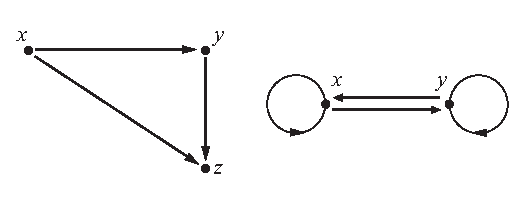
\includegraphics{figps-transitive.eps}
\end{center}
\end{figure}
\end{itemize}
%There are other properties of relations that can be studied, but we will restrict ourselves to these three, as they are the ones pertinent to the study of equivalence relations.

\begin{prog}[\textbf{Properties of Relations}] \label{prog:proprelations} \hfill \\
Let  $A = \{ a, b, c, d \}$ and let $R$ be the following relation on $A$:
\[
R = \{ (a, a), (b, b), (a, c), (c, a), (b, d), (d, b) \}.
\]
Draw a directed graph for the relation $R$ and then determine if the relation $R$ is reflexive on $A$, if the relation $R$ is symmetric, and if the relation $R$ is transitive.
\end{prog}
\hbreak

\endinput
